\section{Entanglement generation}\label{sec:4:entanglement-generation}
If the full state $\rho$ is measured repeatedly but for each measurement the initial setup was slightly different, this effectively is an averaging process over all the variations in the setup.
As mentioned earlier, this averaging mixes the state and for large variations $\Delta \theta$ and $\Delta L$, this process can destroy entanglement.
To see this, we calculate the averaged state $\mean{\rho}$ as
\begin{equation}\label{eq:4:average-density}
  \mean{\rho} = \int_{\infty}^{\infty} \dd \theta_A p(\theta_A) \int_{\infty}^{\infty} \dd \theta_B p(\theta_B) \int_{\infty}^{\infty} \dd L_A p(L_A) \int_{\infty}^{\infty} \dd L_B p(L_B) \ \rho(\theta_A, \theta_B, L_A, L_B)
\end{equation} 
where $p(x)$ is the gaussian probability distribution of the quantity $x$. For both, $\theta$ and $L$, this is distributed around mean $0$ and with standard deviation $\Delta \theta$ and $\Delta L$. $\rho(\theta_A, \theta_B, L_A, L_B)$ is the state of a single measurement, dependent on the parameters $\theta_i$ and $L_i$ of the setup.
This state is very similar as before in \cref{cha:first-look} but with the additional effect of the casimir interactions taken into account.
The initial state $\ket{\psi_0}$ at $t=0$ is given by eq. \eqref{eq:2:initial-state}.
During the time evolution, not only the mutual gravitational interactions between the masses but also the Casimir interactions between the shield and the states has to be taken into account. A state $\ket{\psi^i_{A(B)}}$ ($i = 1, 2$) accumulated the phase $\phi^i_{A(B),\,\mathrm{Cas}}(t)$ during time evolution.
This phase is given by
\begin{equation}
  \phi^i_{A(B),\,\mathrm{Cas}}(t) = \frac{t}{\hbar}
  \begin{cases}
     \frac{3 \hbar c}{8 \pi} \left(\frac{\varepsilon_r - 1}{\varepsilon_r + 2}\right) \frac{R^3}{(L^i_{A(B)})^4} & \text{for large separations (LSL)} \\
    \frac{\hbar c \pi^3}{720} \varphi(\varepsilon_r) \left(\frac{\varepsilon_r - 1}{\varepsilon_r + 1}\right) \frac{R}{(\mathscr{L}^i_{A(B)})^2} & \text{for small separations (PFA)}
  \end{cases}
\end{equation}
where a distinction between the different Casimir-models has been made.
The plate-sphere separations $L^i_{A(B)}$ or $\mathscr{L}^i_{A(B)} = L^i_{A(B)}-R$ are of course dependent on the placement of the particles.
In full generality, they are given by
\begin{equation}
  L^i_{A(B)} = L + L_{A(B)} - \frac{d}{2} \pm \frac{\Delta x_{A(B)}}{2} \sin(\xi + \theta_{A(B)})
\end{equation}
where $\pm$ depends on the considered state and $\xi = \alpha, \beta$ was used as an abbreviation.
The mutual gravitational interaction for states $\ket{\psi^i_A}\otimes\ket{\psi^j_B}$ is given similar to before by the accumulated phase
\begin{equation}
  \phi^{ij}_\mathrm{Grav}(t) = \frac{t}{\hbar} \frac{G M_A M_B}{L^{ij}} .
\end{equation}
The separation between the spheres $L^{ij}$ ($i,j = 1,2$) in full generality is given by
\begin{multline}
  L^{ij} = \sqrt{\left(2L + L_A + L_B \pm \frac{\Delta x_A}{2}\sin(\alpha + \theta_A) \mp \frac{\Delta x_B}{2}\sin(\beta + \theta_B)\right)^2 +} \\ \overline{\left(\frac{\Delta x_A}{2}\cos(\alpha + \theta_A) \pm \frac{\Delta x_B}{2}\cos(\beta + \theta_B)\right)^2}
\end{multline}
Expanding both phases in first order of $\theta_{A(B)} \ll 1$, $L_{A(B)} \ll 1$ (which is feasible as seen later), the averaging in eq. \eqref{eq:4:average-density} can be performed analytically.
It turns out, that all off-diagonal elements of the averaged state $\mean{\rho}$ are given in the form
\begin{equation}
  \mean{\rho_{kl}} = e^{i \Delta \phi_{kl}(t)} \exp{-\frac{(\Delta\theta)^2}{2} (\Delta\phi_{kl,\,\theta})^2 t^2} \exp{-\frac{(\Delta L)^2}{2} (\Delta\phi_{kl,\,L})^2 t^2}
\end{equation}
where all $\Delta \phi$-terms are replacements for rather lengthy linearized phase expressions which depend on the separation $L$, the orientation $\alpha, \beta$, the masses $M_{A(B)}$ and the delocalization size $\Delta x_{A(B)}$.
It becomes evident, that for large times or for large variations in the placement, these off-diagonal elements tend to zero. 
For $t\rightarrow \infty$ or for $\Delta \theta, \Delta L \rightarrow \infty$, this state represents the maximally mixed state with $\tr\rho^2 = 1/4$, which obviously is not entangled.
For large variations in the placement, one therefore expects a loss of entanglement.

The resulting logarithmic negativity of the averaged state $E_N(\mean{\rho})$ was computed numerically for different values of $\Delta \theta$ and $\Delta L$ and is shown in \cref{fig:4:EN-delta-theta}.
\begin{figure}[!htbp]
  \centering
  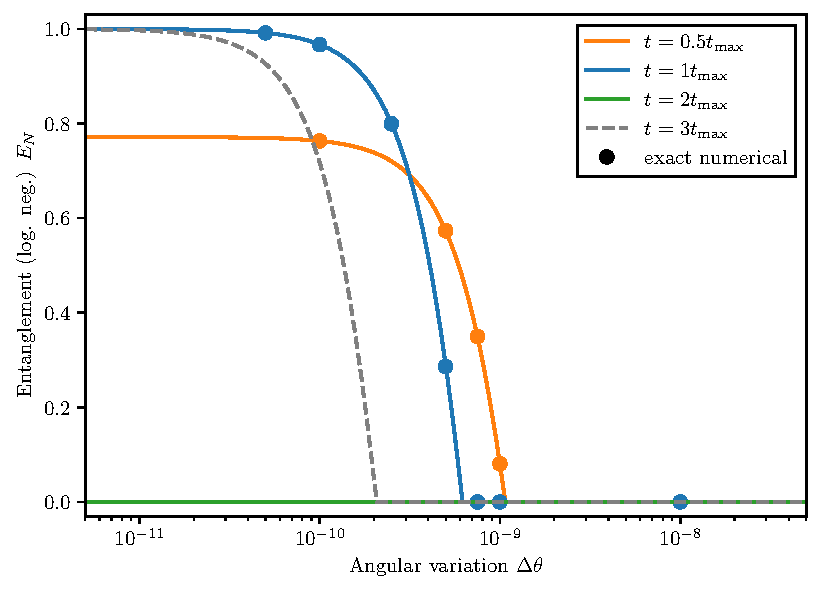
\includegraphics[width=\textwidth]{./../figures/theta-variance/EN-delta-theta.pdf}
  \caption{Entanglement quantified by the logarithmic negativity (eq. \eqref{eq:2:logarithmic-negativity}) dependent on the angular variation $\Delta\theta$. The entanglement is shown at different times, where $t_\mathrm{max}$ is the time of maximal entanglement calculable by eq. \eqref{eq:4:t-max}. Additionally, a few selected exact numerical results are shown to align precisely with the approximated version.}
  \label{fig:4:EN-delta-theta}
\end{figure}
For this figure, the parallel configuration with $\alpha = \beta = 0$ was used with $t_\mathrm{max}$ given by eq. \eqref{eq:2:logarithmic-negativity}as well as 
